In this chapter, we will identify and design a controller for the master motor of the rolling mill. During the operation, this motor will be controlled with a constant reference and it should keep its velocity as steady as possible.

\section{Master motor}
The master motor is the one that pulls the strip and winds it up on a spool. The left motor was chosen as master since its setpoint velocity is higher than that of the right motor. This is necessary since when the strip is compressed to reduce its thickness it extends, which means the speed of the winding motor should be higher than the feeding motor. Figure \ref{fig:LM_RPM_curr} shows the static characteristic of the left motor and table \ref{tab:LM_operating_region} shows the currents and speed for different operating points.

\begin{figure}[htbp]
\centering
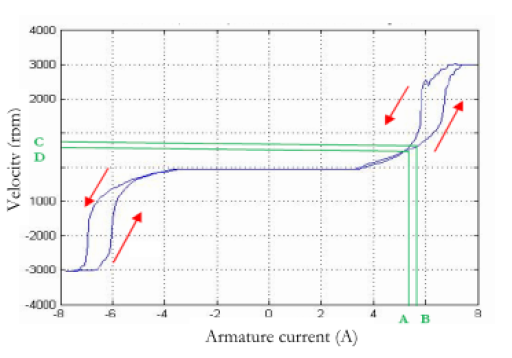
\includegraphics[width = .6\textwidth]{pics/LM_RPM_Current.png}
\caption{Static characteristic of the left motor\label{fig:LM_RPM_curr}}
\end{figure}

\begin{table}[htbp]
	\centering
	\begin{tabular}{rr}
    \toprule
		Armature current [A] & Angular velocity [RPM] \\ \midrule
    5.4 & 530.7 \\
    5.7 & 649.8 \\\bottomrule
	\end{tabular}
	\caption{Operating points of the left motor\label{tab:LM_operating_region}}
\end{table}

\section{Identification of the Transfer Function}
The transfer function of the left motor is identified with a least square approximation using matlab. To do this, the measured velocity is sampled for an input step between the setpoints, since that is the region where we want to linearize the behaviour of the motor. We choose to fit the system with a first order transfer function which is common for a DC motor with big inertial load.

Figure \ref{fig:LM_id} shows the measured and fitted step responses. We see that the system is indeed heavily dominated by a single slow real pole, and that it is well approximated by transfer function \ref{eq:LM_TF}.

\begin{equation}
	LM(s) = \frac{5.398}{3.642S+1}
  \label{eq:LM_TF}
\end{equation}

\begin{figure}[htbp]
\centering
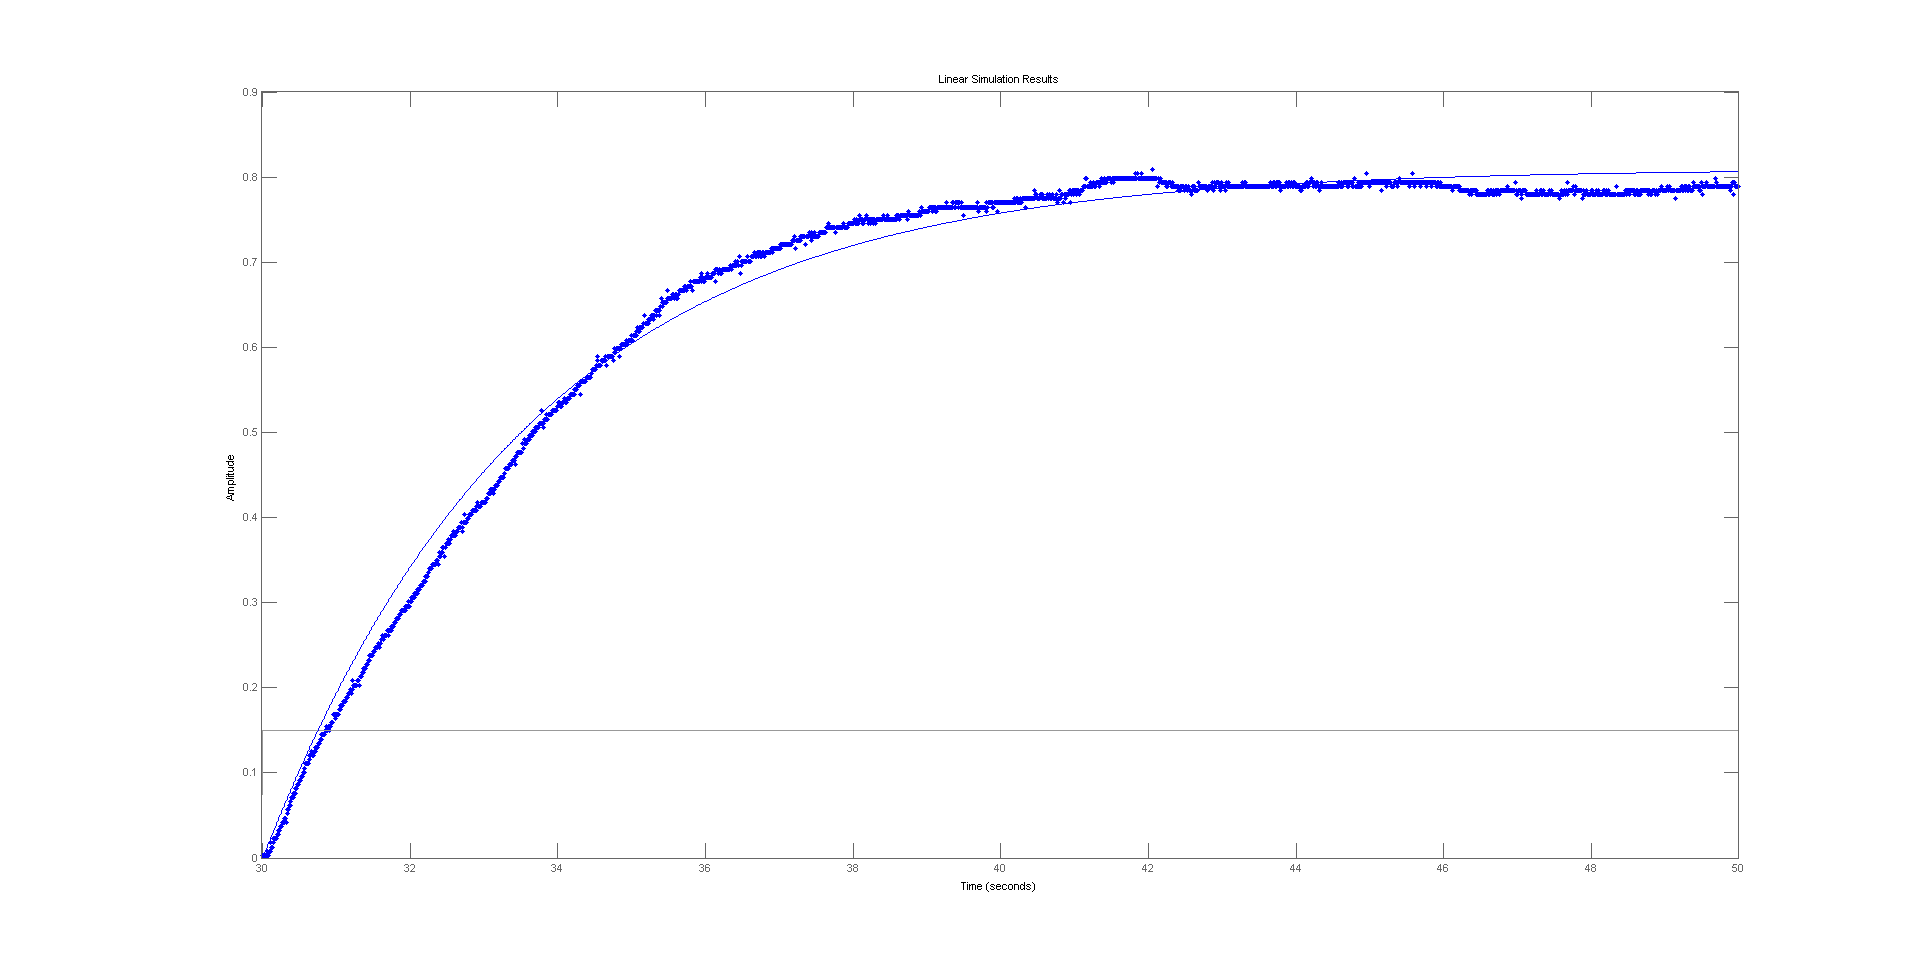
\includegraphics[width = \textwidth]{identification_step_setpoints.png}
\caption{Sampled and fitted step response of the left motor\label{fig:LM_id}}
\end{figure}

\section{Design of a PI Controller}
The master motor is controlled with a constant reference and should keep its velocity as steady as possible despite possible disturbance. For this reason, we choose to control it with a PI controller, which should provide asymptotic stability, zero steady state error, and perturbation rejection.

We use the root locus method to tune the PI controller. First we choose $\frac{K_I}{K_P}$ so that the zero of the controller cancels the pole of the motor. This theoretically ensures that the closed loop has a single negative real pole that can then be arbitrarily placed by adjusting $K_P$. In the following, we detail the calculations used to determine the gains using this method.

First, the transfer functions of the left motor and the PI controller are transformed to make the poles and zeroes immediately visible.
\begin{align*}
	LM(s) &= \frac{5.398}{3.642s+1}\\
				&= \frac{1.482}{s+0.274}\\
\\PI(s) &= K_p + \frac{K_i}{s}\\
    		&= K_p \cdot \frac{s+\frac{K_i}{K_p}}{s}
\end{align*}
To cancel the pole of the motor, we hence use $\frac{K_i}{K_p} = 0.294$.

We then choose $K_P$ using a root locus. The open loop is given by:
\begin{align*}
    OL(s) &= \frac{1.482}{s+0.274} \cdot \frac{s+0.274}{s} \\
					&= \frac{1.482}{s}
\end{align*}

Figure \ref{fig:LM_rl}
\begin{figure}[htbp]
\centering
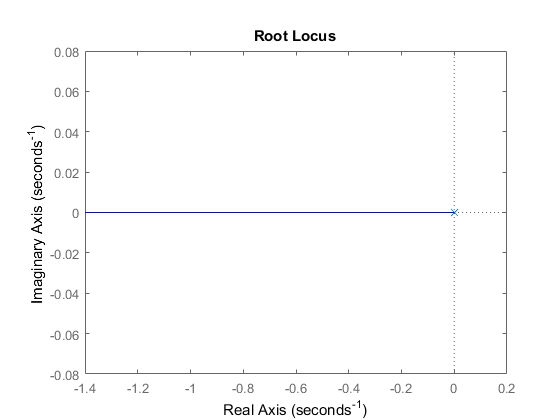
\includegraphics[width = .7\textwidth]{pics/LM_cont_rlocus.png}
\caption{Root locus plot for the left motor with a PI controller\label{fig:LM_rl}}
\end{figure}
shows that $K_P > 0$ can theoretically be chosen arbitrarily. Non linearities, higher order effects and actuator saturation will determine its ideal value.

Figures \ref{fig:LM_SIM_KP050} -- \ref{fig:LM_SIM_KP200}
\begin{figure}[htbp]
\centering
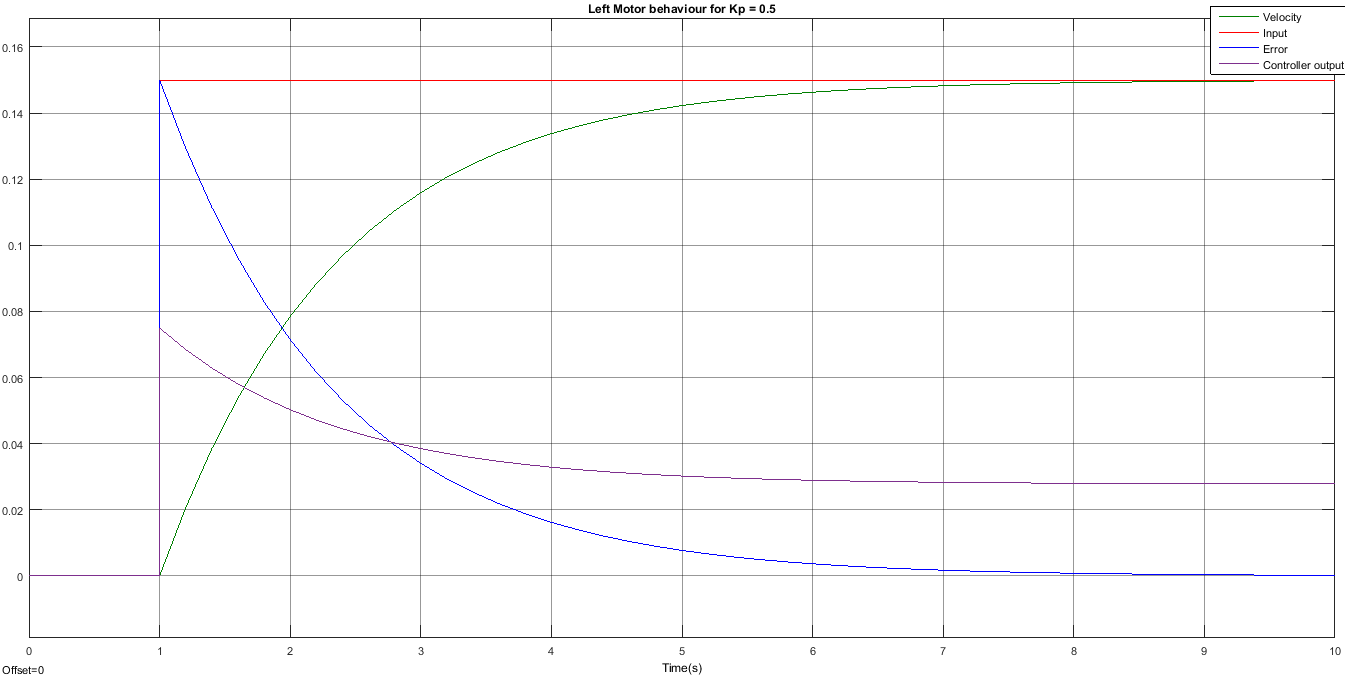
\includegraphics[width = \textwidth]{pics/LM_KP050_Sim.png}
\caption{Simulink simulation of the left motor behaviour for $K_p = 0.5$}
\label{fig:LM_SIM_KP050}
\end{figure}
%
\begin{figure}[htbp]
\centering
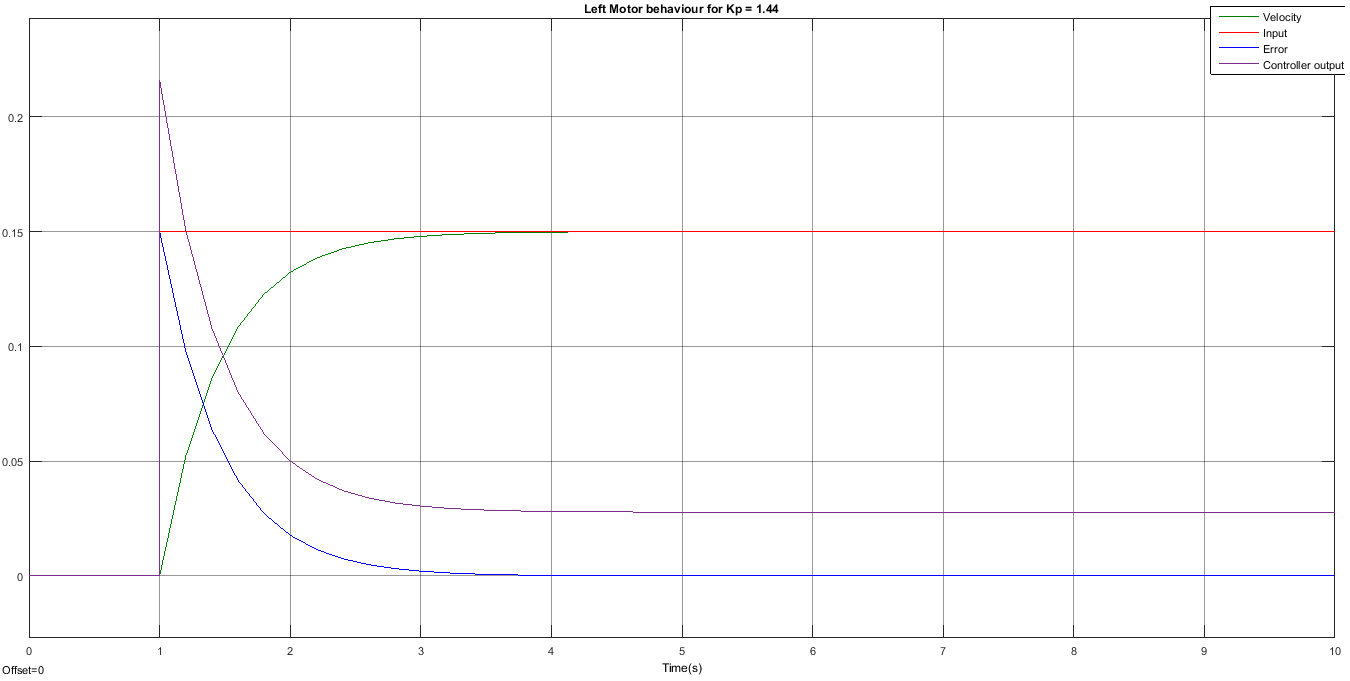
\includegraphics[width = \textwidth]{pics/LM_KP144_Sim.png}
\caption{Simulink simulation of the left motor behaviour for $K_p = 1.44$}
\label{fig:LM_SIM_KP144}
\end{figure}
%
\begin{figure}[htbp]
\centering
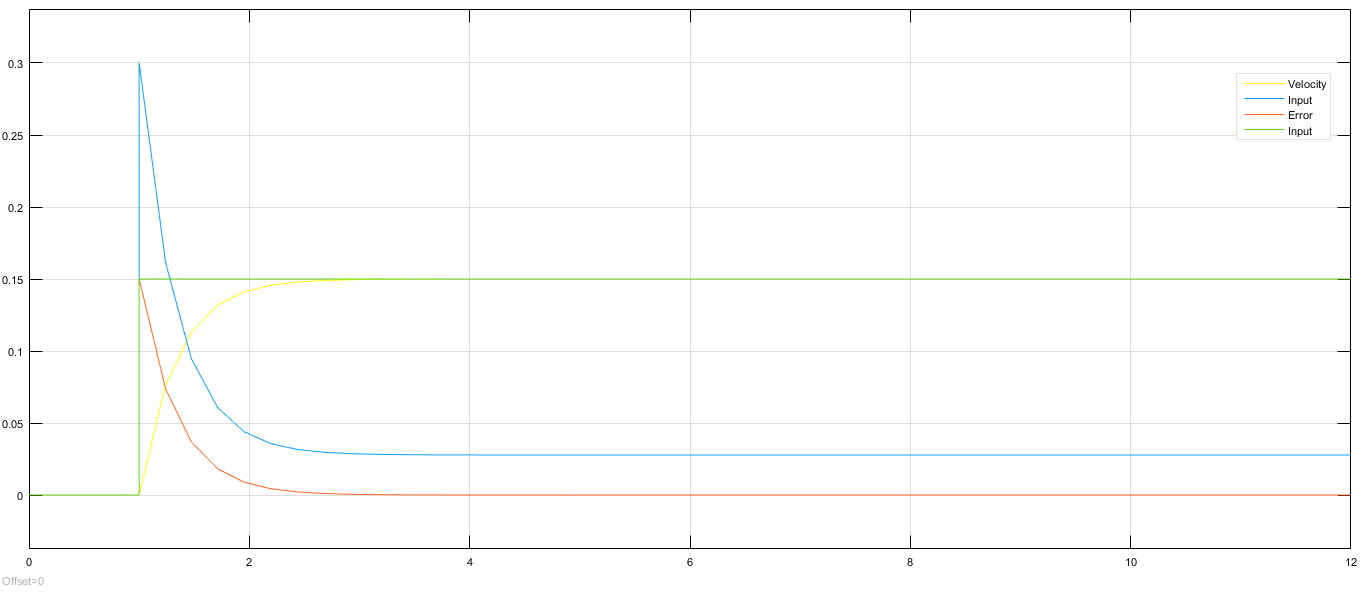
\includegraphics[width = \textwidth]{pics/LM_KP200_sim.png}
\caption{Simulink simulation of the left motor behaviour for $K_p = 2$}
\label{fig:LM_SIM_KP200}
\end{figure}
show the result of simulink simulations for several values of $K_P$. We see that actuator saturation will probably not be the deciding constraint\footnote{The blue curve represents the small signal input on each of the plots. The setpoint value is \SI{2.7}{V} and the input range is [\SI{-10}{V} - \SI{10}{V}].}. We thus need to implement the controller to be able to experimentally tune its gain.

\FloatBarrier
\section{Tuning of the PI Controller}
Figures \ref{fig:LM_KP050} -- \ref{fig:LM_KP200} show experimental runs of the master motor with different values of $K_P$. Based on these measurements $K_P = 1.44$ was chosen. $K_P = 0.5$ has a longer settling time with a larger overshoot than $K_p = 1.44$, and $K_P = 0.5$ has a longer, higher overshoot.  Since $\frac{K_I}{K_P} = 0.294$, $K_I = 0.3954$. None of the simulations have overshoot while all the practical experiments do. This is because the transfer function of the motor was reduced to a first order system while in practice it behaves as a non linear system of higher order.
\begin{figure}[htbp]
\centering
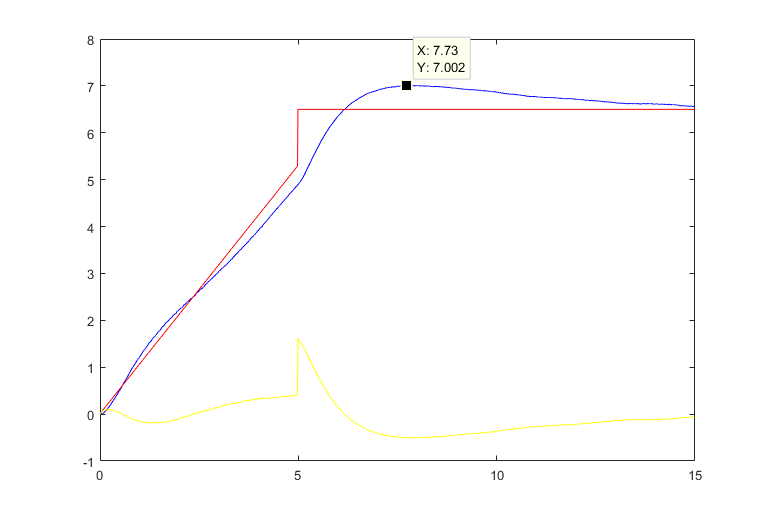
\includegraphics[width = .7\textwidth]{pics/LM_KP050a.png}
\caption{Response of the left motor behaviour for $K_p = 0.5$ to the red curve as input.}
\label{fig:LM_KP050}
\end{figure}
%
\begin{figure}[htbp]
\centering
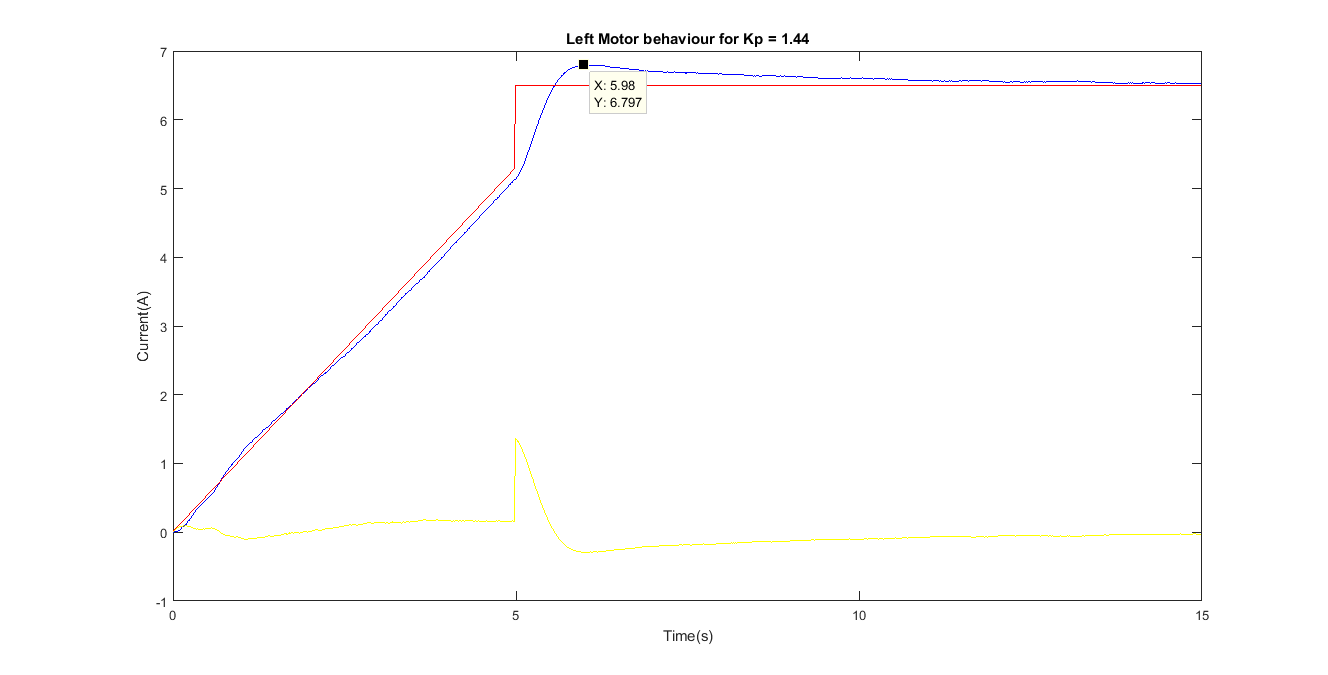
\includegraphics[width = \textwidth]{pics/LM_KP144.png}
\caption{Response of the left motor behaviour for $K_p = 1.44$ to the red curve as input.}
\label{fig:LM_KP144}
\end{figure}
%
\begin{figure}[htbp]
\centering
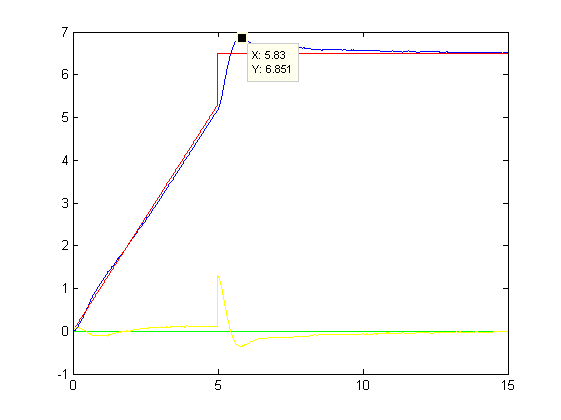
\includegraphics[width = .7\textwidth]{pics/LM_KP200.png}
\caption{Response of the left motor behaviour for $K_p = 2$ to the red curve as input.}
\label{fig:LM_KP200}
\end{figure}

We observe that we indeed obtain zero steady state error, and that disturbances of order higher than 1 seem to not affect the master velocity too much, which is very good.
\section{Conclusion}
We decide to control the master motor with a PI controller and the following values:
\begin{align*}
	K_P = 1.44
	K_I = 0.3954
\end{align*}
This allows us to generate a steady, precise master speed around which we will then modulate the slave speed in order to control the traction of the metallic strip. In the next chapter, we will identify and design a controller for the slave motor, which will serve as an inner loop for the traction control.
